\documentclass[
  aspectratio=1610,
]{beamer}

% chktex-file 26

\usefonttheme{professionalfonts}
\usefonttheme[stillsansseriflarge, stillsansserifsmall]{serif}

%\usetheme{Frankfurt}
%\usecolortheme{dove}

\usepackage{amsmath, amssymb}

\usepackage[MnSymbol]{mathspec}
\defaultfontfeatures{
  Ligatures=TeX,
  Scale=MatchLowercase,
}
\setsansfont{Gill Sans}
\setmainfont{Minion Pro}
\setmonofont{Fira Mono}

\usepackage{xltxtra}
\usepackage{polyglossia}
\setdefaultlanguage{german}

\usepackage{hyperref}

\usepackage{minted}

\setbeamertemplate{navigation symbols}{}

\newcommand{\wplogo}{
\includegraphics[height=2ex]{enwiki.png}}

\author{Martin Darmüntzel}
\title{Einführung in C}
%\subtitle{}
\institute{Universität Rostock}
%\date{6. September 2019}

\begin{document}

\begin{frame}
  \titlepage{}
\end{frame}

% \section{Geschichte}%

\begin{frame}
  \begin{center}
    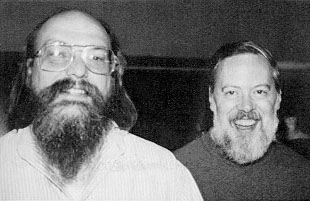
\includegraphics{Ken_Thompson_and_Dennis_Ritchie--1973.jpg}

    Ken Thompson \& Dennis Ritchie
  \end{center}
  \tiny Quelle:
  \url{https://en.wikipedia.org/wiki/File:Ken_Thompson_and_Dennis_Ritchie--1973.jpg}
\end{frame}

\begin{frame}
  \begin{center}
    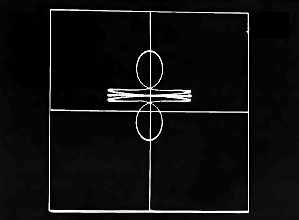
\includegraphics{Space_Travel_Screenshot.png}

    Space Travel
  \end{center}
  \tiny Quelle:
  \url{https://en.wikipedia.org/wiki/File:Space_Travel_Screenshot.png}
\end{frame}

\begin{frame}
  \begin{center}
    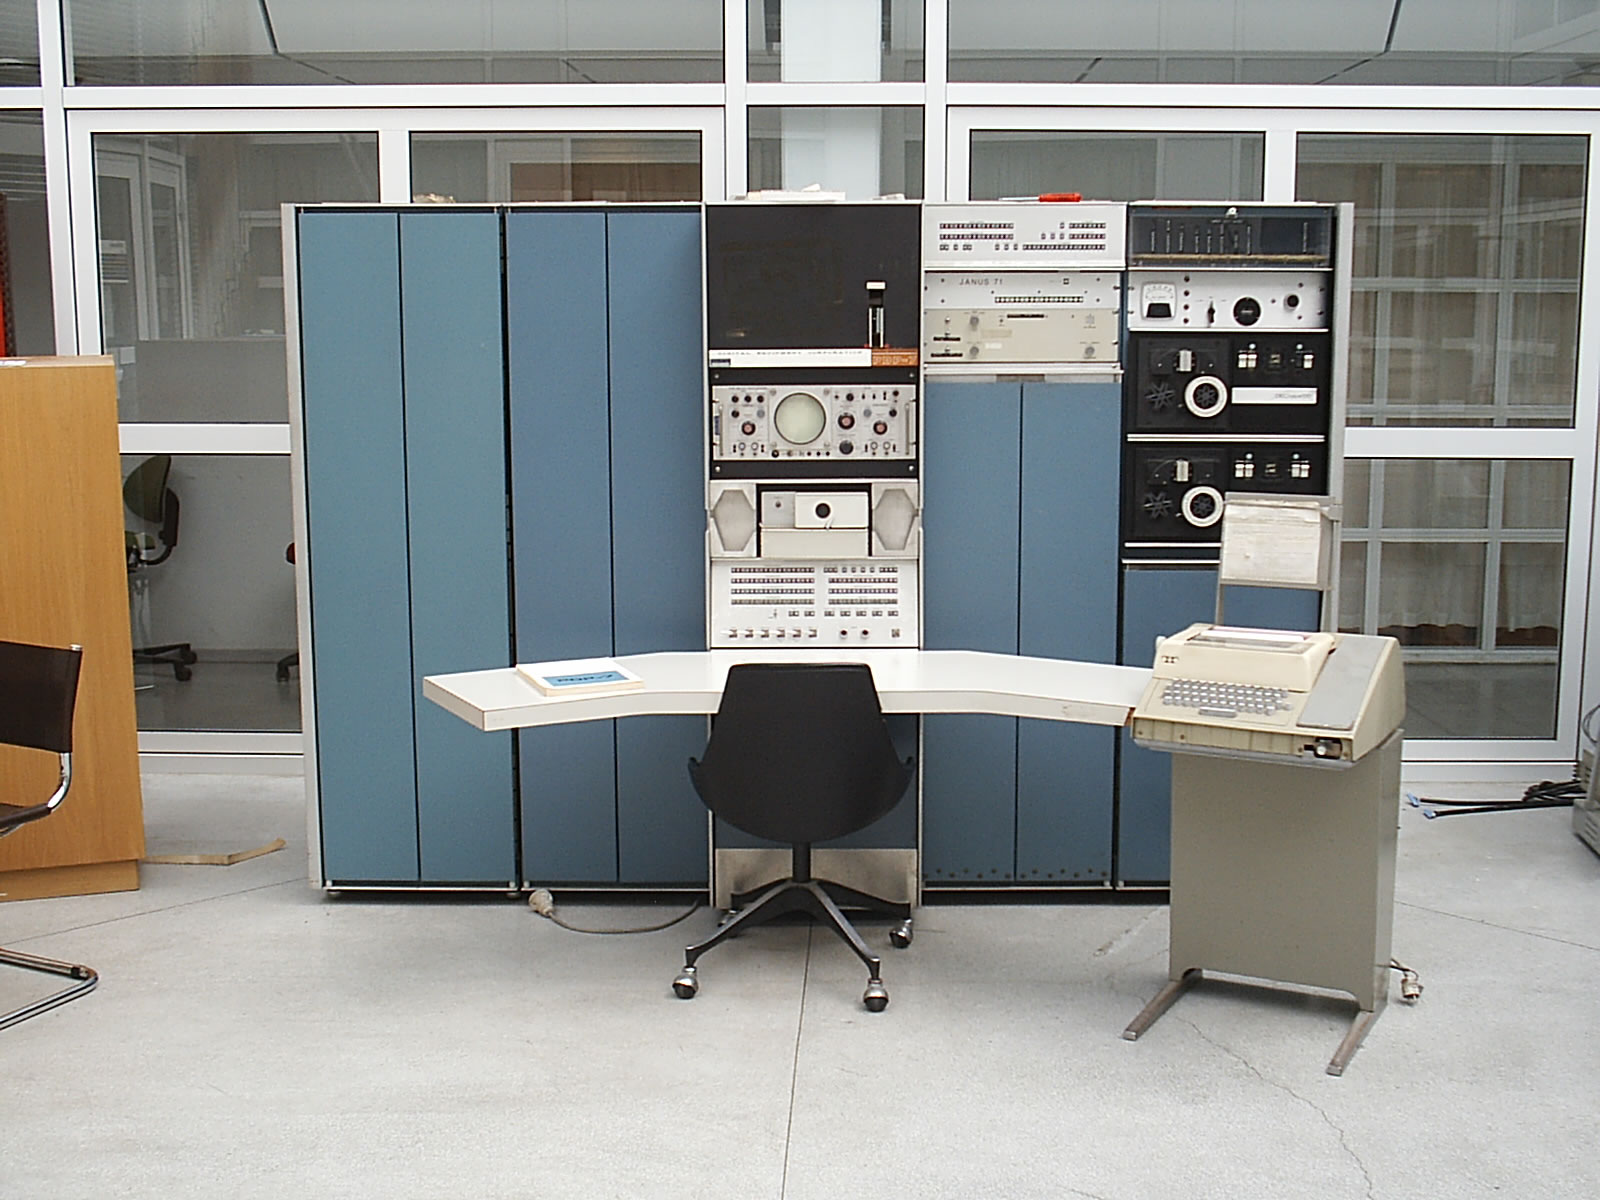
\includegraphics[width=0.75\textwidth]{Pdp7-oslo-2005.jpeg}

    PDP-7
  \end{center}
  \tiny Quelle:
  \url{https://upload.wikimedia.org/wikipedia/commons/5/52/Pdp7-oslo-2005.jpeg}
\end{frame}

\begin{frame}{Programmierprobleme unserer Großeltern}
  \begin{itemize}
    \item viele verschiedene Computer- bzw. Prozessorhersteller
    \item viele verschiedene Architekturen mit verschiedenen Instruktionssätzen

      siehe z.\,B.
      \href{https://en.wikipedia.org/wiki/Comparison_of_instruction_set_architectures}{Comparison
      of instruction set architectures \wplogo}
    \item viele verschiedene Maschinensprachen bzw. Assemblersprachen
    \item[$\rightarrow$] ein Programm für einen PDP-7 lief nicht auf einem Intel-Prozessor
  \end{itemize}

  \pause{}
  \vspace{1em}

  Lösung: Abstraktion durch Hochsprachen

  \begin{itemize}
    \item Fortran (1957)
    \item ALGOL (1958)
    \item LISP (1958)
    \item[$\rightarrow$] C (1972)
  \end{itemize}
\end{frame}

\begin{frame}{Warum C?}
  \begin{itemize}
    \item simple Syntax
    \item flexibel und portierbar
    \item abstrakt genug $\leftrightarrow$ konkret genug („Hochsprachen-Assembler“)
    \item Grundlage für viele wichtige Programme und andere Programmiersprachen
  \end{itemize}
\end{frame}

\begin{frame}{Programmieren im Allgemeinen}
  Mensch schreibt Quelltext
  $\rightarrow$ Compiler produziert Programm aus Maschinencode
  $\rightarrow$ Betriebssystem führt Programm aus

  \pause{}

  \begin{block}{Wichtig}
    Quelltext wird für Menschen geschrieben, nicht für Maschinen!
  \end{block}
\end{frame}

\begin{frame}{Handwerkszeug}
  \begin{itemize}
    \item Quelltext schreiben: Texteditor,
      z.\,B. \texttt{gedit}, \texttt{vim}, \texttt{emacs}
    \item Compiler: \texttt{gcc}, \texttt{clang}, meist einfach nur \texttt{cc}
    \item Programm ausführen: Terminal
  \end{itemize}

  \pause{}

  \begin{block}{Wichtige Basisbefehle im Terminal}
    \begin{description}
      \item[\texttt{pwd}] zeigt das aktuelle Verzeichnis an
      \item[\texttt{ls}] listet den Verzeichnisinhalt auf
      \item[\texttt{cd}] wechselt das Verzeichnis
        \begin{itemize}
          \item \texttt{cd ..} wechselt in das übergeordnete Verzeichnis % chktex
        \end{itemize}
      \item[\texttt{cc}] kompiliert Quelltext
        \begin{itemize}
          \item \texttt{\$ cc hello.c} erzeugt die ausführbare Datei \texttt{a.out}
          \item \texttt{\$ ./a.out} führt sie aus
          \item \texttt{\$ cc -o hello hello.c} erzeugt die ausführbare Datei \texttt{hello}
          \item \texttt{\$ ./hello} führt sie aus
        \end{itemize}
    \end{description}
    Bitte abschreiben!
  \end{block}
\end{frame}

\begin{frame}{Hello, world!}
  \inputminted{c}{hello.c}

  \begin{block}{Aufgabe}
    Öffne einen Texteditor (z.\,B. \texttt{gedit}), schreibe den Quelltext ab und
    speichere ihn in der Datei \texttt{hello.c}.

    Öffne ein Terminal und kompiliere die Datei mittels \texttt{cc hello.c}.

    Führe das erzeugte Programm mittels \texttt{./a.out} aus.
  \end{block}
\end{frame}

\end{document}
